\begin{figure}
\centering
\fbox{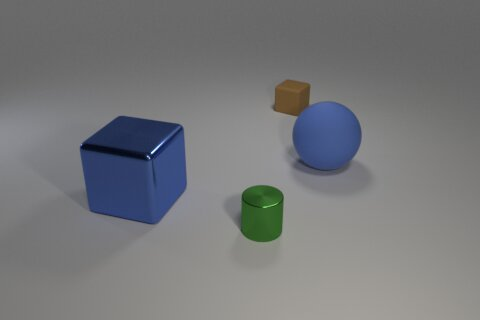
\includegraphics[width=0.533\linewidth]{figures/samples/clevr.jpg}}
\begin{minted}[breaklines]{python}
add(color='green', size='tiny', material='shiny', shape='cylinder', loc=(2.163, -1.384, 0.350))
add(material='metal', rotation=-0.126, shape='cube', loc=(-0.033, -2.456, 0.700), color='blue', size='large')
add(size='large', material='rubber', color='blue', loc=(1.352, 1.165, 0.700), shape='sphere')
add(color='brown', material='matte', shape='cube', size='tiny', loc=(-1.185, 2.816, 0.350), rotation=0.144)
\end{minted}
\caption{\textbf{CLEVR-CoGenT Train Sample.} (\cref{ssec:clevr})}
\label{fig:code_clevr}
\end{figure}